\section{Data Analysis}
Data analysis is the act of analyzing, cleansing, manipulating, and modeling data in order to identify usable information, generate conclusions, and help decision-making[].
Data analysis has several dimensions and approaches, including a wide range of techniques known by various names and applied in a variety of business, science, and social science sectors. [2]
In today's corporate world, data analysis plays an important part in making decisions more scientific and assisting firms in operating more efficiently[].
Data mining is a type of data analysis technique that focuses on statistical modeling and knowledge discovery for predictive rather than purely descriptive purposes,
whereas \ac{BI} is a type of data analysis that focuses on aggregation and is primarily concerned with business information, more on this later.

\subsection{Procedure for analyzing data}
The term \textit{``analysis''} refers to the process of breaking down a whole into its constituent parts for closer evaluation.
Data analysis is the act of getting raw data and then transforming it into information that users can utilize to make decisions.
Data is gathered and processed in order to answer questions, test hypotheses, or refute theories[].

\begin{figure}[ht]
    \centering
    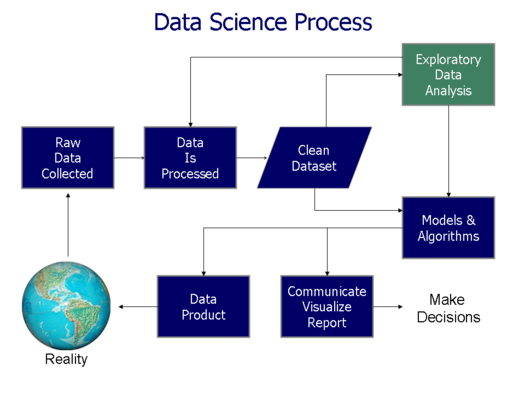
\includegraphics[width=\textwidth]{content/chapter_1/images/Data_visualization_process_v1.png}
    \caption{Data science process flowchart \cite{Book:doing_data_science}}
    \label{fig:data-science-flowchart}
\end{figure}

There are various distinct phases that can be identified, these are iterative in the sense that input from later phases may lead to further effort in earlier ones.
Similar stages can be found in the CRISP framework, which is used in data mining. 

\subsection{What is Data?}
We talked a lot about data in the last section and while it is important that we can analyze and understand data, but what is data?
Understanding what data is it's a prerequisite for being able to use it properly, perhaps the most important thing as far as we're concerned
\subsection{Data Cleaning}
\subsection{Data Transformation}
\subsection{Data Reduction}